\documentclass[12pt]{article}
\usepackage[margin=1in]{geometry}
\usepackage{arev}
\usepackage{pgfplots}
\usepackage[inline]{enumitem}
\usetikzlibrary{calc}
\pgfplotsset{compat=newest}

\begin{document}
\section*{Quiz}
On each slope field, sketch any three particular solutions and find the corresponding

\begin{figure}[!hbt]
	\centering

	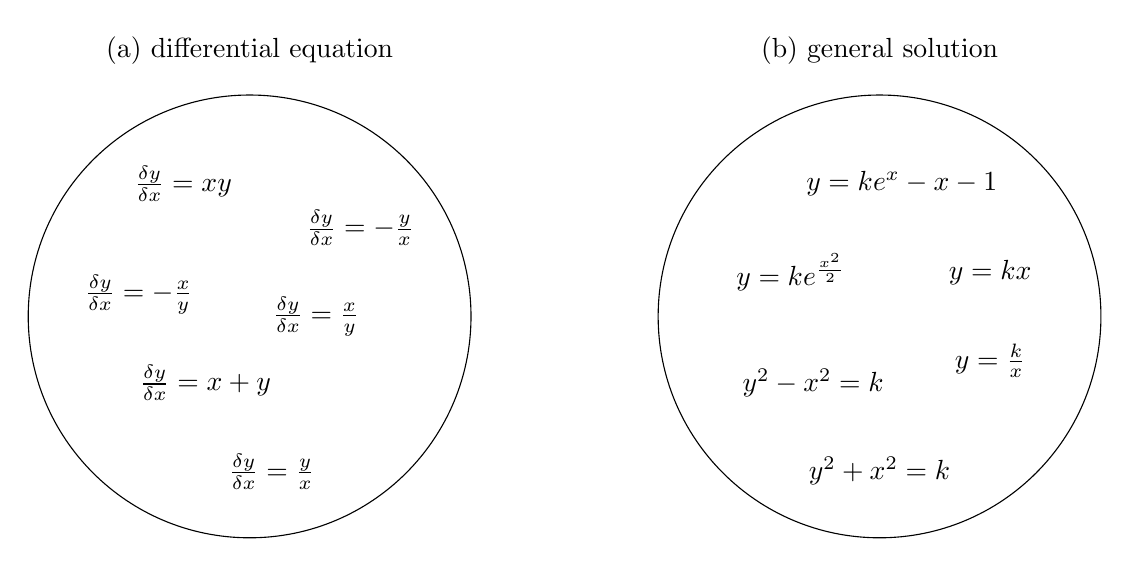
\begin{tikzpicture}
		\def\r{80pt}
		\coordinate (left) at (-4,0);
		\coordinate (right) at (4,0);
		\node at ($(left) + (0,1.2*\r)$) {(a) differential equation};
		\node at ($(right) + (0,1.2*\r)$) {(b) general solution};

		\draw (left) circle [radius=\r];
		\draw (right) circle [radius=\r];

        \newcommand\dd[2]{\frac{\delta#1}{\delta#2}}

		\node at ($(left) + (-0.2*\r,-0.3*\r)$) {$\dd{y}{x} = x+y$};
		\node at ($(left) + (-0.3*\r,0.6*\r)$) {$\dd{y}{x} = xy$};
		\node at ($(left) + (0.1*\r,-0.7*\r)$) {$\dd{y}{x} = \frac{y}{x}$};
		\node at ($(left) + (0.5*\r,0.4*\r)$) {$\dd{y}{x} = -\frac{y}{x}$};
		\node at ($(left) + (0.3*\r,0*\r)$) {$\dd{y}{x} = \frac{x}{y}$};
		\node at ($(left) + (-0.5*\r,0.1*\r)$) {$\dd{y}{x} = -\frac{x}{y}$};

		\node at ($(right) + (0.1*\r,0.6*\r)$) {$y=ke^x-x-1$};
		\node at ($(right) + (-0.4*\r,0.2*\r)$) {$y=ke^{\frac{x^2}{2}}$};
		\node at ($(right) + (0.5*\r,0.2*\r)$) {$y=kx$};
		\node at ($(right) + (0.5*\r,-0.2*\r)$) {$y=\frac{k}{x}$};
		\node at ($(right) + (-0.3*\r,-0.3*\r)$) {$y^2-x^2=k$};
		\node at ($(right) + (0*\r,-0.7*\r)$) {$y^2+x^2=k$};
	\end{tikzpicture}

	\vspace{1cm}

	\def\width{6.6cm} \def\height{6.6cm}
    \def\domainMin{-3} \def\domainMax{3}
    \newcommand\slopefield[1] {
    \begin{tikzpicture}[
        trim axis left, trim axis right,
        declare function={ dydx(\x,\y) = #1;
        }]
        \begin{axis}[
            xmin=\domainMin, xmax=\domainMax, ymin=\domainMin, ymax=\domainMax,
            width=\width, height=\height,
            tick align=outside,
            xtick={\domainMin,...,\domainMax}, ytick={\domainMin,...,\domainMax},
            xticklabel=\empty, yticklabel=\empty,
            major tick length=0.1cm,
            every tick/.append style={thin, black},
            ]
            \coordinate (O) at (axis cs:0,0);
            \coordinate (X) at (axis cs:1,0);
            \coordinate (Y) at (axis cs:0,1);
        \end{axis}

        % Get axis coordinate system and plot slope field
        \begin{scope}[x={($(X)-(O)$)}, y={($(Y)-(O)$)}, shift={(O)}]
        \def\numSlopes{16}
        \pgfmathsetmacro{\scale}{(\domainMax-\domainMin)/25}
        \pgfmathsetmacro{\hx}{(\domainMax-\domainMin)/(\numSlopes+1)} % +2 to account for the slopes at the domain edge that aren't drawn
        \pgfmathsetmacro{\hy}{(\domainMax-\domainMin)/(\numSlopes+1)}
        \pgfmathsetmacro{\totalSlopes}{\numSlopes^2-1}
        \foreach \i [evaluate=\i as \x using \domainMin+\i*\hx] in {1,...,\numSlopes} {
            \foreach \j [evaluate=\j as \y using \domainMin+\j*\hy] in {1,...,\numSlopes} {
                \pgfmathsetmacro{\slope}{dydx(\x, \y)}
                \pgfmathsetmacro{\dx}{\scale/sqrt((\slope)^2+1)}
                \pgfmathsetmacro{\dy}{\slope*\dx}
                \draw[thin] ({\x-\dx/2},{\y-\dy/2})--({\x+\dx/2},{\y+\dy/2});
            }
        }

        % Draw additional axis lines
        \draw[black!60] (\domainMin,0)--(\domainMax,0);
        \draw[black!60] (0,\domainMin)--(0,\domainMax);
        
        % Question number
        \node[anchor=north west, fill=white] at (\domainMin,\domainMax) {\stepcounter{qnumber}\theqnumber.};
        \end{scope}
    \end{tikzpicture}
    }

    \newcounter{qnumber}

	\slopefield{\x+\y} \hspace{\fill} \slopefield{\x*\y} \hspace{\fill} \slopefield{\y/\x} % top row
	\vspace{1cm}
	\slopefield{-\y/\x} \hspace{\fill} \slopefield{\x/\y} \hspace{\fill} \slopefield{-\x/\y} % bottom row
\end{figure}

\end{document}
